\documentclass{beamercours}


\title{Théorie des Jeux et Théorie des Langages}
\author{Matthieu Boyer}
\date{18 Janvier 2024}

\usetikzlibrary{automata, arrows, calc, matrix, positioning}
\definecolor{vulm}{HTML}{7d1dd3}
\definecolor{yulm}{HTML}{ffe500}
\usepackage{caption}

\usepackage{tcolorbox}
\tcbuselibrary{theorems}
\NewTcbTheorem[auto counter, number within=section]{définition}{Définition}%
 {colback=yulm!10, colframe=vulm!45!black, fonttitle=\bfseries}{def}

\NewTcbTheorem[use counter from=définition]{théorème}{Théorème}%
 {colback=yulm!10!white, colframe=vulm!65!black, fonttitle=\bfseries}{thm}

\NewTcbTheorem[use counter from=définition]{propositionfr}{Proposition}%
 {colback=yulm!10!white, colframe=vulm!25!black, fonttitle=\bfseries}{propo}

\NewTcbTheorem[use counter from=définition]{corollaire}{Corollaire}%
 {colback=yulm!10, colframe=vulm!35!black, fonttitle=\bfseries}{cor}

\NewTcbTheorem[use counter from=définition]{lemme}{Lemme}%
 {colback=yulm!10, colframe=vulm!15!black, fonttitle=\bfseries}{lemme}

\NewTcbTheorem[use counter from=définition]{remarque}{Remarque}%
 {colback=yulm!10, colframe=vulm!65!black, fonttitle=\bfseries}{rem}

\begin{document}
\maketitle
\begin{frame}{Plan}\tableofcontents\end{frame}

\section{Introduction}
\begin{frame}
    \frametitle{Introduction}
    \begin{figure}[h]
        \centering
        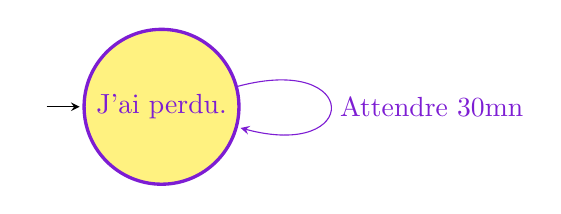
\begin{tikzpicture}[shorten >=1pt,node distance=1cm,>={stealth}, initial text = ,
            every state/.style={draw=vulm,very thick,fill=yulm!50, text = vulm}, accepting/.style={accepting by arrow, double}]
            \node[state, initial] (q) {J'ai perdu.};
            \path[->, vulm] (q) edge[loop right] node [right] {Attendre 30mn} (q);
        \end{tikzpicture}
        \caption{\textsc{Le Jeu}}
        \label{fig:dfa:lejeu}
    \end{figure}
    

\end{frame}
% \begin{frame}
%     \frametitle{Introduction}
%     \only<1>{Un jeu à plusieurs joueurs est, de manière informelle, une abstraction d'un jeu ressemblant par exemple au Tarot : chaque joueur, à son tour, va choisir, parmi un éventail de coups possibles, celui qu'il souhaite effectuer, modifiant alors l'état du jeu.}
%     \only<2>{On limite en quelque sorte les transitions possibles de l'état de jeu selon l'état et selon les règles du jeu. Le manque d'informations d'un joueur sur les mains de ses adversaires limite aussi la description directe du jeu avec du non-déterminisme. \\
%         On s'intéresse donc ici à des manières de décrire les jeux par les automates et les grammaires formelles.}
% \end{frame}

\section{Jeux et Automates}
\subsection{Premières Définitions}
\begin{frame}
\frametitle{Notion de Jeu}
\begin{définition}{Première définition de Jeu suivant \cite{game-rep-automata}}{}
Un jeu est un triplet $\left(P, A_{i}, \succeq_{i}\right)$ où $P$ est un ensemble de joueurs, $A_{i}$ est un ensemble d'actions pour le joueur $i \in P$ et $\succeq_{i}$ est une relation de préférence pour le joueur $i$.
\end{définition}
\visible<2>{Pour le \textsc{Dilemme du Prisonnier}: $P = \left\{1, 2\right\}$, et $\forall i, A_{i} = \left\{A, N\right\}$}
\end{frame}

\begin{frame}
\frametitle{Représentation Extensive}
\only<1>{\begin{définition}{Description Extensive}{}
    La description extensive d'un jeu est son arbre de possibilités.
    \end{définition}}
\only<2>{\begin{figure}
        \centering
        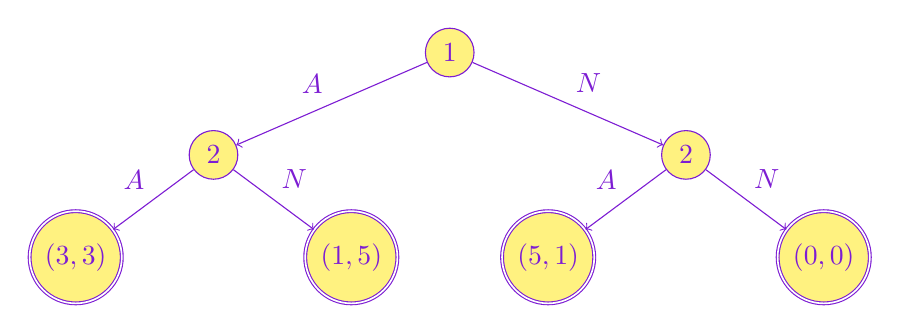
\begin{tikzpicture}[level distance=1.3cm,
                level 1/.style={sibling distance=6cm},
                level 2/.style={sibling distance=3.5cm}]
            \tikzstyle{every node}=[circle, minimum size = .5cm,draw = vulm, fill = yulm!50, text = vulm]
            \node {1}
            child[vulm] {node {2}
                    child[vulm] {node[double] {$(3, 3)$} edge from parent[->] node[above left, draw = none, fill = none] {$A$}}
                    child[vulm] {node[double] {$(1, 5)$} edge from parent[->] node[above right, draw = none, fill = none] {$N$}}
                    edge from parent[->] node[above left, draw = none, fill = none] {$A$}
                }
            child[vulm] {node {2}
                    child[vulm] {node[double, minimum size = .5cm] {$(5, 1)$} edge from parent[->] node[above left, draw = none, fill = none] {$A$}}
                    child[vulm] {node[double, minimum size = .5cm] {$(0, 0)$} edge from parent[->] node[above right, draw = none, fill = none] {$N$}}
                    edge from parent[->] node[above right, draw = none, fill = none] {$N$}
                };
        \end{tikzpicture}
        \caption{Représentation Extensive du Jeu du \textsc{Dilemme du Prisonnier} à information totale.}
        \label{fig:gametree:full_info_pridi}
    \end{figure}}
\end{frame}

\begin{frame}
\frametitle{Information Imparfaite}
\only<1>{\begin{définition}{Information d'un Jeu}{}
    On parle de jeu à information imparfaite, lorsque le joueur actuel n'a pas d'informations sur les coups des joueurs précédents. On rajoute l'information possédée par un joueur sur l'arbre de jeu.
    \end{définition}}
\only<2>{\begin{figure}
        \centering
        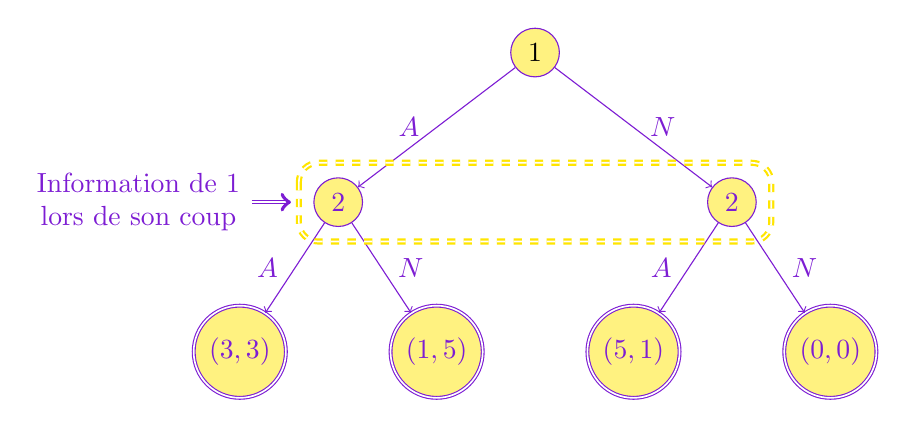
\begin{tikzpicture}[level distance=1.9cm,
                level 1/.style={sibling distance=5cm},
                level 2/.style={sibling distance=2.5cm}]
            \tikzstyle{every node}=[circle,draw = vulm, fill = yulm!50]
            \node(0) {1}
            child[vulm] {node {2}
                    child[vulm] {node[double] {$(3, 3)$} edge from parent[->] node[left, draw = none, fill = none] {$A$}}
                    child[vulm] {node[double] {$(1, 5)$} edge from parent[->] node[right, draw = none, fill = none] {$N$}}
                    edge from parent[->] node[left, draw = none, fill = none] {$A$}
                }
            child[vulm] {node {2}
                    child[vulm] {node[double] {$(5, 1)$} edge from parent[->] node[left, draw = none, fill = none] {$A$}}
                    child[vulm] {node[double] {$(0, 0)$} edge from parent[->] node[right, draw = none, fill = none] {$N$}}
                    edge from parent[->] node[right, draw = none, fill = none] {$N$}
                };
            \draw[dashed,rounded corners=7, double, yulm, thick = 2pt]($(0-1)+(-.5,.5)$)rectangle($(0-2)+(.5,-.5)$);
            \tikzstyle{every node} = []
            \node at ($(0-1) + (-1,.)$)[label ={[align = center, vulm]left : Information de $1$\\ lors de son coup}]{};
            \draw[->, double, distance = 5pt, vulm]($(0-1) + (-1.1,.)$)--($(0-1)+(-.6,.)$);
        \end{tikzpicture}
        \caption{Représentation Extensive du Jeu du \textsc{Dilemme du Prisonnier} à information imparfaite.}
        \label{fig:gametree:impinfopridi}
    \end{figure}
}
\end{frame}

\begin{frame}
\frametitle{Partie sur un Jeu}
\begin{définition}{Partie sur un Jeu}{}
Une partie sur un jeu est une suite d'états de ce jeu, ou, de manière équivalente, une suite de coups $s_{0}s_{1}\ldots s_{k}$ tels que :
\begin{itemize}
    \item $\forall i, s_{2i} \in A_{0}$ et $s_{2i + 1} \in A_{1}$.
    \item $\nexists s_{k + 1} \in A_{i}$ où $i = 1$ si $k \equiv 0 \mod 2$ et $i = 0$ sinon.
\end{itemize}
\end{définition}
\end{frame}


\subsection{Jeux sur les Automates}
\begin{frame}
\frametitle{Jeu d'un Automate}
\only<1>{\begin{définition}{Jeu d'un Automate}{}
    Si $A = \left(Q, \Sigma, \delta, q_{0}, F\right)$ est un automate, on se donne $G_{A}$ un jeu sous représentation extensive à deux joueurs \textsc{Tatiana} et \textsc{Pierre}. Dans ce jeu, \textsc{Tatiana} joue des états de $Q$ et \textsc{Pierre} joue des lettres de $\Sigma$.
    \end{définition}}
\only<2>{
    \begin{définition}{Règles du Jeu}{}
    Les règles du jeu pour chaque joueur sont les suivantes : si \textsc{Tatiana} joue $q \in \Sigma$ alors \textsc{Pierre} doit jouer $s$ tel que $\delta(q, s) \neq \emptyset$ sinon il perd.
    \end{définition}}
\only<3>{
    \begin{itemize}
        \item Si $A$ est déterministe, $G_{A}$ est équivalent à un jeu à information parfaite.
        \item A l'inverse, si $A$ n'est pas déterministe, on définit des ensembles d'informations récursivement.
    \end{itemize}}
\end{frame}

\begin{frame}
    \frametitle{Un Exemple Déterministe}
    \only<1>{\begin{figure}
            \centering
            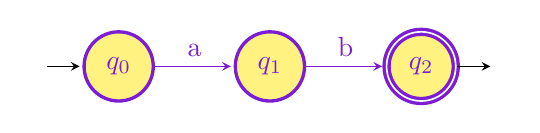
\begin{tikzpicture}[shorten >=1pt,node distance=1cm,>={stealth}, initial text = ,
                every state/.style={draw=vulm,very thick,fill=yulm!50, text = vulm}, accepting/.style={accepting by arrow, double}]
                \node[state, initial] (q_0) {$q_{0}$};
                \node[state] (q_1) [right=of q_0] {$q_{1}$};
                \node[state, accepting] (q_2) [right = of q_1] {$q_{2}$};
                \path[->, vulm] (q_0) edge node [above] {a} (q_1)
                (q_1) edge node [above] {b} (q_2);
            \end{tikzpicture}
            \caption{Un Automate Déterministe}
            \label{fig:dfa1}
        \end{figure}}
    \only<2>{
        \begin{figure}
            \centering
            \resizebox{8.0cm}{!}{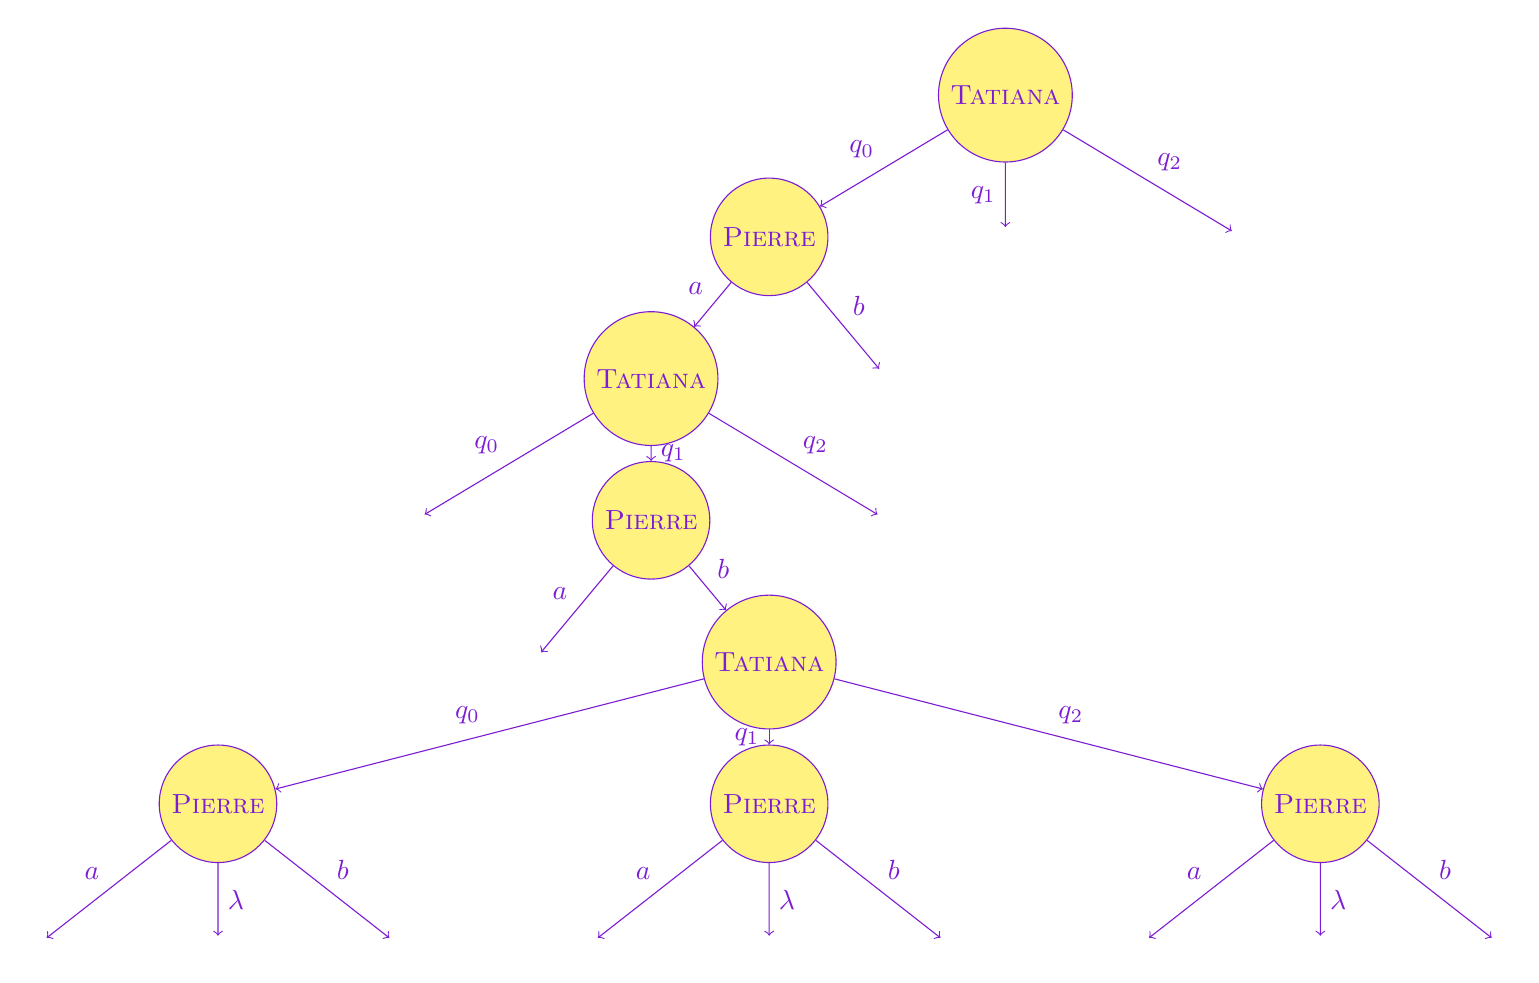
\begin{tikzpicture}[level distance=1.8cm,
                        level 1/.style={sibling distance=3cm},
                        level 2/.style={sibling distance=3cm},
                        level 3/.style={sibling distance=3cm},
                        level 4/.style={sibling distance=3cm},
                        level 5/.style={sibling distance=7cm},
                        level 6/.style={sibling distance=2.3cm}]
                    \tikzstyle{every node}=[draw = none, fill = none]
                    \node[circle, draw = vulm, fill=yulm!50, text = vulm] {\textsc{Tatiana}}
                    child[vulm] {node[circle, draw = vulm, fill=yulm!50] {\textsc{Pierre}}
                    child[vulm] {node[circle, draw = vulm, fill=yulm!50] {\textsc{Tatiana}}
                    child[vulm] {node {} edge from parent[->] node[above left] {$q_{0}$}}
                    child[vulm] {node[circle, draw = vulm, fill=yulm!50] {\textsc{Pierre}}
                    child[vulm] {node {} edge from parent[->] node[above left] {$a$}}
                    child[vulm] {node[circle, draw = vulm, fill=yulm!50] {\textsc{Tatiana}}
                    child[vulm] {node[circle, draw = vulm, fill=yulm!50] {\textsc{Pierre}}
                    child[vulm] {node {} edge from parent[->]node[above left]{$a$}}
                    child[vulm] {node {} edge from parent[->]node[right]{$\lambda$}}
                    child[vulm] {node {} edge from parent[->]node[above right]{$b$}}
                    edge from parent[->] node[above left] {$q_{0}$}}
                    child[vulm] {node[circle, draw = vulm, fill=yulm!50] {\textsc{Pierre}}
                    child[vulm] {node {} edge from parent[->]node[above left]{$a$}}
                    child[vulm] {node {} edge from parent[->]node[right]{$\lambda$}}
                    child[vulm] {node {} edge from parent[->]node[above right]{$b$}}
                    edge from parent[->] node[left] {$q_{1}$}}
                    child[vulm] {node[circle, draw = vulm, fill=yulm!50] {\textsc{Pierre}}
                    child[vulm] {node {} edge from parent[->]node[above left]{$a$}}
                    child[vulm] {node {} edge from parent[->]node[right]{$\lambda$}}
                    child[vulm] {node {} edge from parent[->]node[above right]{$b$}}
                    edge from parent[->] node[above right] {$q_{2}$}}
                    edge from parent[->] node[above right] {$b$}}
                    edge from parent[->] node[right] {$q_{1}$}
                    }
                    child[vulm] {node {} edge from parent[->] node[above right] {$q_{2}$}}
                    edge from parent[->] node[above left] {$a$}
                    }
                    child[vulm] {node {} edge from parent [->] node[above right] {$b$}}
                    edge from parent[->] node[above left] {$q_{0}$}}
                    child[vulm] {node {} edge from parent [->] node[left] {$q_{1}$}}
                    child[vulm] {node {} edge from parent [->] node[above right] {$q_{2}$}};
                \end{tikzpicture}}
            \caption{Représentation Extensive du Jeu à Information Parfaite de l'automate figure \ref{fig:dfa1}}
            \label{fig:gametree:dfa1}
        \end{figure}}
\end{frame}

\section{Théorèmes de Reconnaissance}
\subsection{Stratégies Gagnantes et Langages}
\begin{frame}
\frametitle{Stratégies}
\only<1>{La stratégie d'un joueur assigne une action choisie par le joueur pour chaque historique des coups dans lequel c'est à son tour de jouer. \\
    L'historique d'un joueur est l'ensemble des actions qu'il peut choisir de faire durant la partie.
}
\only<2>{\begin{définition}{Stratégie}{}
    Une stratégie pour \textsc{Pierre} définie par $w \in \Sigma^{\star}$ est telle que \textsc{Pierre} joue les lettres de $w$ indépendamment de ce que \textsc{Tatiana} joue.
    \end{définition}}
\only<3>{
    \begin{définition}{Stratégie Gagnante}{}
    Une stratégie $w$ est gagnante pour \textsc{Pierre} si \textsc{Tatiana} n'a pas de coup valide et où son dernier coup est un état final de $A$.\\
    On pose :
    \begin{itemize}
        \item $S\left(G_{A}\right)^{n}$ l'ensemble des stratégies gagnantes de longueur $n$ pour Pierre
        \item $L(A)^{n}$ l'ensemble des mots de longueur $n$ reconnus par $A$
    \end{itemize}
    \end{définition}}
\end{frame}

\begin{frame}
\frametitle{Théorème de Reconnaissance}
\begin{théorème}{Reconnaissance des Stratégies}{}
$S(G_{A})^{n} = L(A)^{n}$
\end{théorème}
\end{frame}

\subsection{Non-Déterminisme}
\begin{frame}
\frametitle{Non-Déterminisme ?}
\only<1>{\begin{définition}{Jeu d'un NFA}{}
    Etant donné un automate non-déterministe $A$, on définit :
    \begin{itemize}
        \item $P$ un ensemble de deux joueurs où \textsc{Tatiana} joue des états et \textsc{Pierre} des lettres.
        \item Un ensemble $I$ d'ensembles d'informations $B$, où on définit $\delta\left(q, s\right) = B$ lorsqu'il y a du non-déterminisme dans la transition.
        \item Des relations de préférence $\succeq_{i}$ entre deux transitions $\delta_{1}, \delta_{2}$ où $\delta_{1} \succeq \delta_{2}$ si et seulement si $d\left(\delta_{1}\right) \leq d(\delta_{2})$.
    \end{itemize}
    \end{définition}}
\only<2>{\begin{figure}
        \centering
        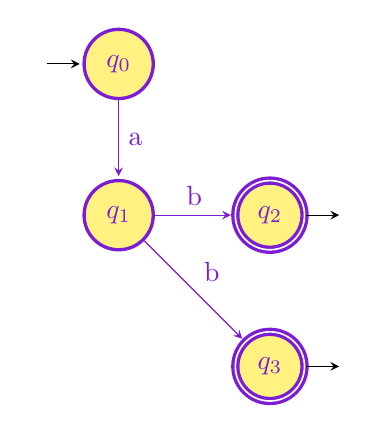
\begin{tikzpicture}[shorten >=1pt,node distance=1cm,>={stealth}, initial text = ,
            every state/.style={draw=vulm,very thick,fill=yulm!50, text = vulm}, accepting/.style={accepting by arrow, double}]
            \node[state, initial] (q_0) {$q_{0}$};
            \node[state] (q_1) [below=of q_0] {$q_{1}$};
            \node[state, accepting] (q_2) [right=of q_1] {$q_{2}$};
            \node[state, accepting] (q_3) [below=of q_2] {$q_{3}$};
            \path[->, vulm] (q_0) edge node [right] {a} (q_1)
            (q_1) edge node [above] {b} (q_2)
            (q_1) edge node [above right] {b} (q_3);
        \end{tikzpicture}
        \caption{Un Automate Non-Déterministe}
        \label{fig:nfa1}
    \end{figure}}
\only<3>{
    \begin{figure}
        \centering
        \resizebox{10.5cm}{!}{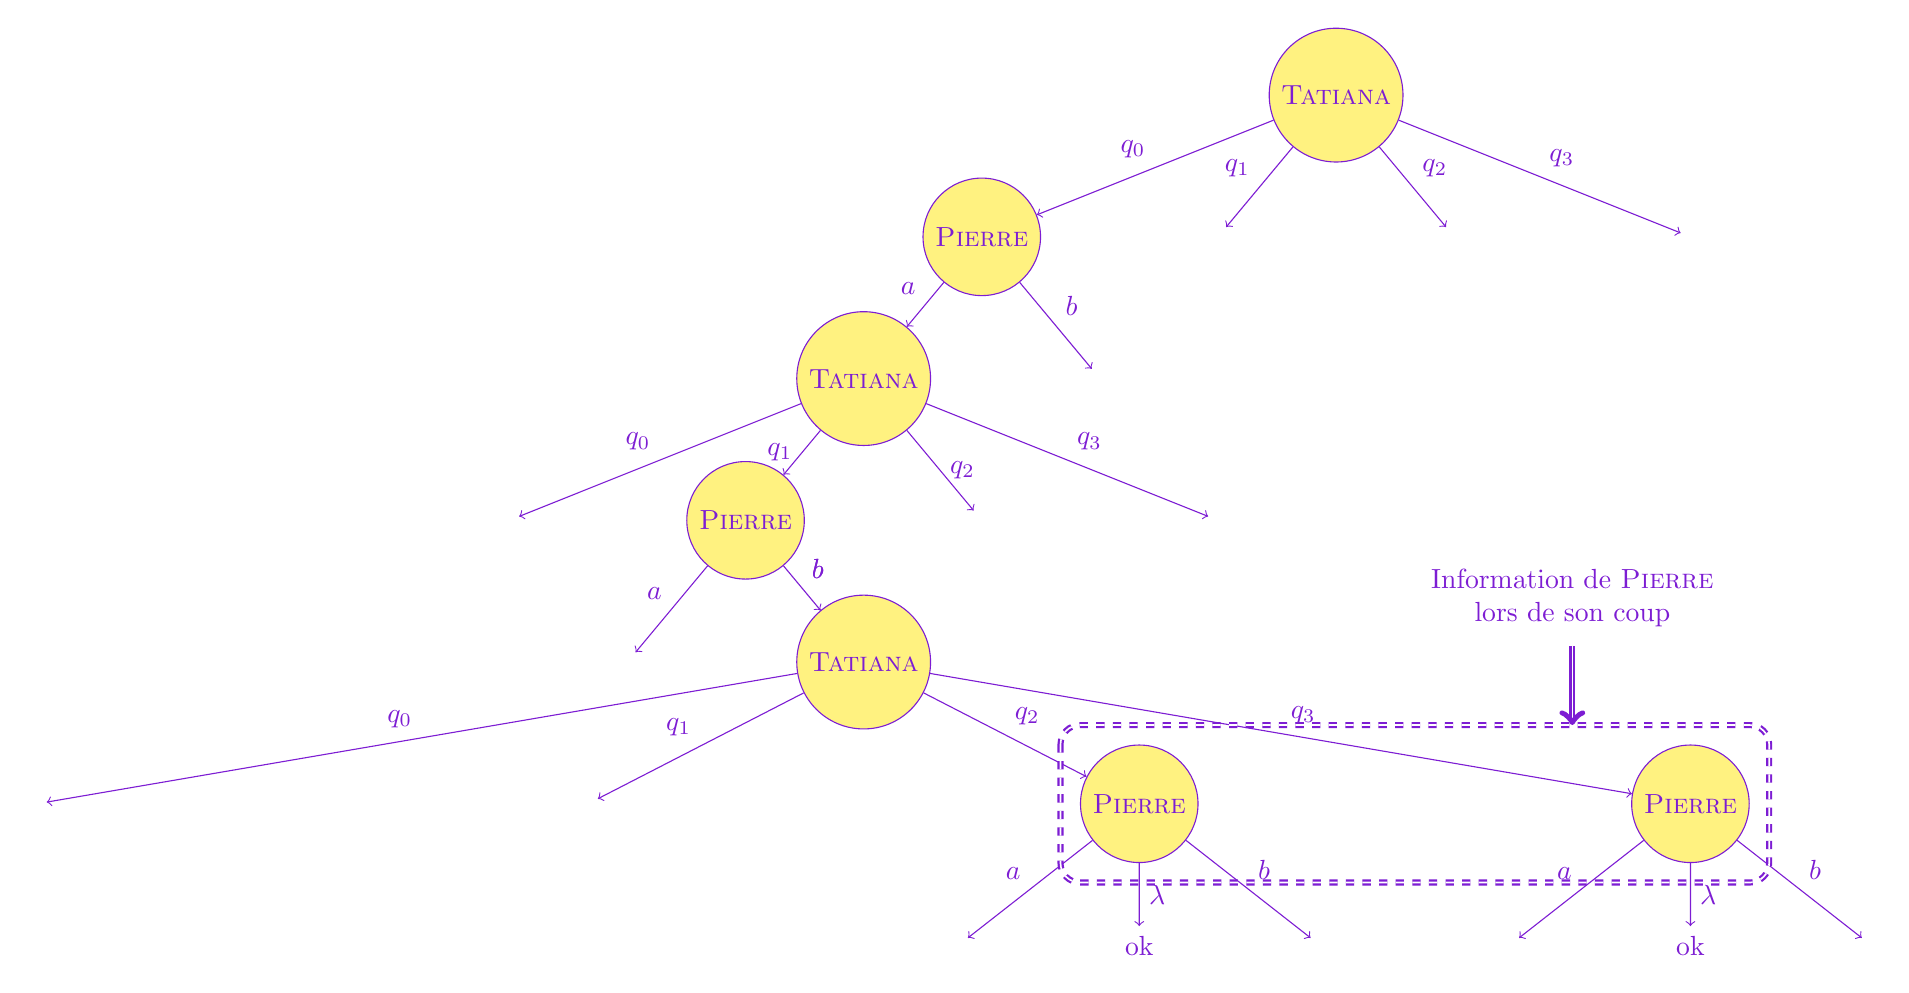
\begin{tikzpicture}[level distance=1.8cm,
                    level 1/.style={sibling distance=3cm},
                    level 2/.style={sibling distance=3cm},
                    level 3/.style={sibling distance=3cm},
                    level 4/.style={sibling distance=3cm},
                    level 5/.style={sibling distance=7cm},
                    level 6/.style={sibling distance=2.3cm}
                ]
                \tikzstyle{every node}=[draw = none, fill = none]
                \node[circle, draw = vulm, fill=yulm!50, text = vulm] (0) {\textsc{Tatiana}}
                child[vulm] {node[circle, draw = vulm, fill=yulm!50] {\textsc{Pierre}}
                child[vulm] {node[circle, draw = vulm, fill=yulm!50] {\textsc{Tatiana}}
                child[vulm] {node {} edge from parent[->] node[above left] {$q_{0}$}}
                child[vulm] {node[circle, draw = vulm, fill=yulm!50] {\textsc{Pierre}}
                child[vulm] {node {} edge from parent[->] node[above left] {$a$}}
                child[vulm] {node[circle, draw = vulm, fill=yulm!50] {\textsc{Tatiana}}
                child[vulm] {node {} edge from parent[->] node[above left] {$q_{0}$}}
                child[vulm] {node {} edge from parent[->] node[above left] {$q_{1}$}}
                child[vulm] {node[circle, draw = vulm, fill=yulm!50](l) {\textsc{Pierre}}
                child[vulm] {node {} edge from parent[->]node[above left]{$a$}}
                child[vulm] {node {ok} edge from parent[->]node[right]{$\lambda$}}
                child[vulm] {node {} edge from parent[->]node[above right]{$b$}}
                edge from parent[->] node[above right] {$q_{2}$}}
                child[vulm] {node[circle, draw = vulm, fill=yulm!50](r) {\textsc{Pierre}}
                child[vulm] {node {} edge from parent[->]node[above left]{$a$}}
                child[vulm] {node {ok} edge from parent[->]node[right]{$\lambda$}}
                child[vulm] {node {} edge from parent[->]node[above right]{$b$}}
                edge from parent[->] node[above right] {$q_{3}$}}
                edge from parent[->] node[above right] {$b$}
                edge from parent[->] node[above right] {$b$}}
                edge from parent[->] node[left] {$q_{1}$}
                }
                child[vulm] {node {} edge from parent[->] node[right] {$q_{2}$}}
                child[vulm] {node {} edge from parent[->] node[above right] {$q_{3}$}}
                edge from parent[->] node[above left] {$a$}
                }
                child[vulm] {node {} edge from parent [->] node[above right] {$b$}}
                edge from parent[->] node[above left] {$q_{0}$}}
                child[vulm] {node {} edge from parent [->] node[above left] {$q_{1}$}}
                child[vulm] {node {} edge from parent [->] node[above right] {$q_{2}$}}
                child[vulm] {node {} edge from parent [->] node[above right] {$q_{3}$}};

                \draw[dashed, rounded corners=7, thick = 2pt, double, draw = vulm]($(l)+(-1,1)$)rectangle($(r)+(1,-1)$);
                \node at ($(l) + (5.5,2)$)[label ={[align = center, vulm]above : Information de \textsc{Pierre}\\ lors de son coup}]{};
                \draw[->, double, thick = 5pt, distance = 5pt, vulm]($(l) + (5.5,2.)$)--($(l)+(5.5,1)$);
            \end{tikzpicture}}
        \caption{Représentation Extensive du Jeu à Information Imparfaite de l'Automate Non-Déterministe Précédent}
        \label{fig:gametree:nfa1}
    \end{figure}}
\end{frame}
\begin{frame}
\frametitle{Théorème de Reconnaissance}
    \begin{théorème}{Information et Reconnaissance}{}
    Tout jeu à information imparfaite est équivalent, au sens de la reconnaissance des langages, à un jeu à information totale.
    \end{théorème}
\end{frame}

\section{Jeux et Grammaires}
\subsection{Jeux Hors-Contexte, Machine de Turing, Automates à Pile}
\begin{frame}
\frametitle{Définitions}
\only<1>{\begin{définition}{Jeu Hors-Contexte}{}
    Un Jeu Hors-Contexte est un triplet $G = \scalar{\Sigma, R, T}$ où $\Sigma$ est un alphabet fini, $R \subseteq \Sigma \times \Sigma^{+}$ est un ensemble fini de règles et $T$ est un automate représentant un langage régulier cible.
    \end{définition}}
\only<2-4>{\begin{itemize}
        \item\only<2>{ Une partie du jeu $G$ est jouée par deux joueurs \textsc{Tatiana} et \textsc{Pierre}. Une partie consiste, à chaque étape, à appliquer une des règles de $R$ à un mot donné sur $\Sigma$. A chaque étape, \textsc{Tatiana} choisit une position dans le mot et \textsc{Pierre} choisit une règle de $R$ associée.}
              \only<3>{Un état du jeu $C$ est une paire $(w, i)$ où $w$ est un mot et $i \leq \abs{w}$ est la position courante. Un choix de position de la configuration $(a_{1}\ldots a_{n}, i)$ est un entier $j \leq n$, un choix de règle consiste à remplacer $a_{j}$ par un mot $u$ tel qu'on a $a_{j} \rightarrow u$ dans $R$. On appelle configuration résultante la configuration $\left(a_{1}\ldots a_{j-1}ua_{j+1}\ldots a_{n}, j\right)$ obtenue. }
              \only<4>{Une partie sur $w$ commence dans la configuration initiale $C_{0} = \left(w, 1\right)$ et s'arrête ou bien lorsque le mot résultat est dans $L(T)$ auquel cas \textsc{Tatiana} gagne ou bien lorsque la position choisie par \textsc{Tatiana} est un terminal auquel cas \textsc{Pierre} gagne.}
    \end{itemize}}
\only<5>{\begin{définition}{Stratégie Gagnante}{}
    On dit que \textsc{Tatiana} a une stratégie gagnante en $\left(w, i\right)$ lorsque quelque soient les coups de \textsc{Pierre}, une configuration de $L(T)$ est atteinte en un nombre fini de coups. On dit que \textsc{Tatiana} gagne $\left(G, w\right)$ si \textsc{Tatiana} a une stratégie gagnante dans $G$ sur $w$.
    \end{définition}}
\end{frame}

\begin{frame}
\frametitle{Reconnaissance de la Victoire}
\begin{théorème}{Reconnaissance de la Victoire}{}
Soit $M$ une machine de Turing bornée en espace par $s(n)$. On peut construire un jeu de sorte que pour tout mot $w = a_{1}\ldots a_{n}$, on ait :
\[
    M \text{ accepte } w \Leftrightarrow \textsc{Tatiana} \text{ gagne } (G, \$q_{0}a_{1}\ldots a_{n}\sqcup^{s(n) - n}\#)
\]
\end{théorème}
\end{frame}

\begin{frame}
\frametitle{Equivalence Hors-Contexte}
\only<1>{\begin{définition}{Système à Pile Alternant}{}
    Un système à pile alternant est un quadruplet $\mathcal{P} = \scalar{S = S_{T} \cup S_{P}, \Gamma, \delta, F}$ i.e. un automate à pile sans entrée avec des états existentiels et universels. On note ici les configurations de cet automate entre crochets $\left[q, u\right]$ pour les distinguer des configurations d'un jeu. On dit qu'une configuration est gagnante si \textsc{Tatiana} peut toujours atteindre une configuration finale sur le jeu, quels que soient les choix de \textsc{Pierre}.
    \end{définition}
}
\only<2>{\begin{théorème}{Equivalence Hors-Contexte}{}
    On peut réduire un système à pile à un jeu hors-contexte et réciproquement en temps polynômial.
    \end{théorème}}
\end{frame}

\subsection{Langage de Description des Jeux de Cartes}
\begin{frame}
\frametitle{Prérequis}
\begin{définition}{Langage de Description}{}
\begin{itemize}
    \item \only<1>{On note $P$ l'ensemble des joueurs.
    \item On appelle \emph{emplacement de carte} une position notée $LA$ dans le jeu où un nombre de cartes peut être posé.
          \begin{itemize}
              \item $P$ mains $H$, une par joueur, notées $HI$, et on notera $HX$ la main du joueur courant, et $HA$ les mains de tous les joueurs.
              \item Un jeu ordonné de cartes $D = \left\{X_{Y} \mid \left(X, Y\right)\in \onen{13} \times \onen{4}\right\}$.
              \item Un certain nombre d'emplacements $TK$ sur la table.
          \end{itemize}}
          \only<2>{On définit de même des emplacements notés $KA$ de jetons pour les jeux à mise. Chaque joueur $I$ en possède deux notés $KI0$ et $KI1$.
    \item On décompose le jeu en plusieurs phases, qui se déroulent, par joueur, en rebouclant (après la dernière phase, on reprend la première). À chaque phase, durant son tour, un joueur peut jouer un nombre variable de règles. }
          \only<3>{Son tour s'arrête lorsque :
              \begin{enumerate}
                  \item Il a \texttt{fini}, il revient alors en jeu à la prochaine phase.
                  \item Il passe à la \texttt{suite}, il revient alors en jeu, dans la même phase, une fois que les tours des autres joueurs sont finis.
                  \item Il est \texttt{sorti} du jeu, il a perdu la partie et ne peut plus jouer.
                  \item Il a \texttt{gagné} la partie, auquel cas la partie s'arrête.
              \end{enumerate}
              Tant qu'il reste des joueurs à la \texttt{suite}, on reboucle.}
          \only<4>{Un jeu s'arrête lorsque toutes les phases ont été jouées ou que tous les joueurs sont \texttt{sortis}.}
\end{itemize}
\end{définition}
\end{frame}

\begin{frame}
    \frametitle{Deux Exemples de Description}
    \only<1>{
        \begin{table}
            \centering
            \caption{Règles de la Grammaire du \textsc{Uno}}
            \label{table:grammar_uno}
            \begin{tabular}{c}
                \toprule
                \texttt{montrer}, \texttt{même couleur}, $T0$, \texttt{jouer}\\
                \midrule
                \texttt{montrer}, \texttt{même valeur}, $T0$, \texttt{jouer}\\
                \midrule
                \texttt{piocher}, \texttt{suite}\\
                \midrule
                \texttt{oblig\_a}, $\lambda$, \texttt{gagne}\\
                \bottomrule
            \end{tabular}
        \end{table}
    }
    \only<2>{
        \begin{table}
            \centering
            \caption{Règles de la Grammaire du \textsc{Texas Hold'Em Poker}}
            \label{table:grammar_poker}
            \resizebox{8.0cm}{!}{\begin{tabular}{lr|lr}
                \toprule
                Phase & Règle & Phase & Règle\\
                \midrule
                Phase 1 & \texttt{oblig\_nocond\_parier}, $\lambda$, $\lambda$ & Phase 2 & \texttt{oblig\_jetons}, $KX1$, $<$, $KA1$\\
                (Premier pari) & \texttt{nodonc\_parier}, $=$, $KA1$& (Vérifier paris) & \texttt{sorti} \\
                & \texttt{uniq\_nocond}, \texttt{next}& & \\
                & \texttt{uniq\_nocond\_fini} & & \\
                \midrule
                Phrase 3 & \texttt{piocher}, $D \times 1$ & Phase 4 & \texttt{nocond\_parier}, $\geq$, $KA1$\\
                (Flop) & \texttt{poser}, $D\times 3$, $T0$ & (Deuxième pari) & \texttt{uniq\_nocond\_suite}\\
                & & & \texttt{uniq\_nocond\_fini} \\
                \midrule
                Phase 5 & \texttt{oblig\_jetons}, $KX1$, $<$, $K$ & Phase 6 & \texttt{piocher}, $D \times 1$\\
                (Vérifier paris) & \texttt{sorti} & (Turn) & \texttt{poser}, $D\times 1$, $T0$\\
                \midrule
                Phase 7 & \texttt{nodonc\_parier}, $\geq$, $KA1$ & Phase 8 & \texttt{oblig\_jetons}, $KX1$, $<$, $KA1$\\
                (Troisième pari) & \texttt{uniq\_nocond\_suite} & (Vérifier paris) & \texttt{sorti}\\
                & \texttt{uniq\_nocond\_fini}\\
                \midrule
                Phase 9 & \texttt{piocher}, $D \times 1$ & Phase 10 & \texttt{nodonc\_parier}, $\geq$, $KA1$\\
                (River) & \texttt{poser}, $D\times 1$, $T0$ & (Dernier Pari) & \texttt{uniq\_nocond\_suite}\\
                & & & \texttt{uniq\_nocond\_fini}\\
                \midrule
                Phase 11 & \texttt{oblig\_jeton}, $KX1$, $<$, $KA1$ & Phase 12 & \texttt{oblig\_jouer}, $HX + T0$, $>$\\
                (Vérifier paris) & \texttt{sorti} & (Showdown) & $HA + T0$\texttt{\_gain}, $KA1$\\
                \bottomrule
            \end{tabular}}
        \end{table}
    }

\end{frame}

\section*{Conclusion}
\begin{frame}
    \frametitle{Conclusion}
    \begin{figure}[h]
        \centering
        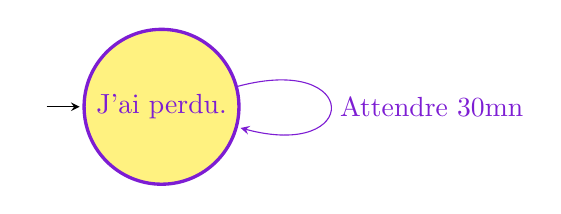
\begin{tikzpicture}[shorten >=1pt,node distance=1cm,>={stealth}, initial text = ,
            every state/.style={draw=vulm,very thick,fill=yulm!50, text = vulm}, accepting/.style={accepting by arrow, double}]
            \node[state, initial] (q) {J'ai perdu.};
            \path[->, vulm] (q) edge[loop right] node [right] {Attendre 30mn} (q);
        \end{tikzpicture}
        \caption{\textsc{Le Jeu}}
        \label{fig:dfa:lejeu}
    \end{figure}
    

\end{frame}
\begin{frame}
    \frametitle{Bibliographie}

    \begin{thebibliography}{7}
        \scriptsize
        \bibitem{game-rep-automata} A-Games: using game-like representation for representing finite automatas \textit{Cleyton Slaviero, Edward Hermann Haeusler}
        \bibitem{card-game-lang} A Card Game Description Language, \textit{Jose M. Font, Tobias Mahlmann, Daniel Manrique, and Julian Togelius}
        \bibitem{cfgames} Active Context-Free Games, \textit{Anca Muscholl, Thomas Schwentick, and Luc Segoufin}
        \bibitem{game-design-automata} Computing Game Design with Automata Theory, \textit{Noman Sohaib Qureshi et al}
        \bibitem{cfgames-sum} Summary for Context Free Games, \textit{Lukáš Holík, Roland Meyer and Sebastian Muskalla}
        \bibitem{permut-grammar} Permutational Grammar for free word order languages, \textit{Mats Eeg-Olofsson and Bengt Sigurd}
        \bibitem{timed-automatas-games} Timed Automata for Video Games and Interaction, \textit{Jaime Arias, Raphael Marczak, Myriam Desainte-Catherine}
    \end{thebibliography}


\end{frame}

\end{document}